\section{音声認識}
音声認識は、音声合成とは逆に、文章を読み上げている音声ファイルからその文章を予想するものです。例えばGoogleのGoogle Homeはまさにこれです。「1時間後に起こして」と声を発すると、内部でそれが文字列に変換されます。その後その文字列を解析してアラームを設定します。
音声認識のためのソフトウェアとしてJuliusというものを使います。入力は音声で出力は文字列になります(図\ref{})。

\begin{figure}[H]
\begin{center}
    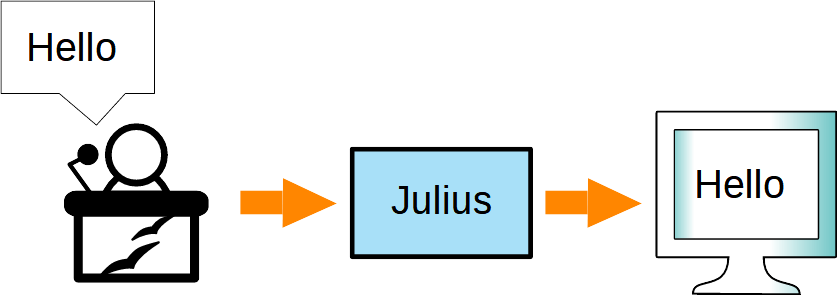
\includegraphics[width=\linewidth]{images/chap06/text06-img002.png}
    \caption{Juliusの入出力}
    \label{Juliusの入出力}
\end{center}
\end{figure}

\begin{tcolorbox}[title=\useOmetoi]
\begin{enumerate}
\item 音声認識とはなんですか。50字以内で説明してください。\\
\underline{答え.\hspace{0.8\linewidth}}
\end{enumerate}
\end{tcolorbox}